% !TEX program = xelatex
% Stony Brook University
% Thesis & Dissertation Template
% Based on Guidelines for the Preparation of Theses and Dissertations - Electronic Submissions
% http://grad.stonybrook.edu/academics/thesis_dissertation_guidelines.php
\documentclass[%
    12pt,  % Size 12 font is recommended by the guidelines
    letterpaper,
    oneside,  % You should NOT add any blank pages to your document
    notitlepage,
%    pagesize,  % No explicit requirement of the paper size by the guidelines
%    parskip=false,  % The first line of each paragraph should be indented using a standard tab indent. What's a standard tab???
%    numbers=noendperiod, % 2.3.1 vs 2.3.1. (no dot after the last chapter number)
%    toc=bibliography, % Bibliography appears in Table of Contents (without a number)
%    toc=listof,  % List of Figures and List of Tables appear in Table of Contents
%    version=last,  % Use latest version of the KOMA-Script
%    chapterprefix=on  % Prefix to chapters
]{report}

\usepackage[]{stonybrook}
\usepackage{lipsum}

%%% Packages
\usepackage[table]{xcolor} 
\usepackage{booktabs}  % Nice tables
\usepackage[autostyle]{csquotes}
\usepackage{longtable}
\usepackage{listings}
\usepackage{algpseudocode}
\usepackage{algorithm}
\usepackage{multirow}
\usepackage{siunitx}
\usepackage{tocbasic}
%%%

% ##############################################
% Start: Floating Object Customization
% ##############################################
%

% Extended support for captions of figures and tables etc.
\usepackage{float}  % Extendes support for floating objects (tables, figures), adds the [H] placing option (\begin{figure}[H]) which palces it "Here".
\usepackage{subcaption}
%

% #######################
% End: Floating Object Customization
% #######################

% Package for PDF features such as bookmarks and hyperlinks. 
\usepackage[%
bookmarks, % Create bookmarks
bookmarksopen=true, % Unfold bookmatk tree in PDF viewer when document is opened
bookmarksopenlevel=1, % Level of unfolding
bookmarksnumbered=true, % Number bookmarks
hidelinks, % do not highlight hyperlinks -- looks ugly
% Ansicht beim Öffnen
pdfpagelabels=true, % See manual...
plainpages=false, % See manual...
hyperfootnotes=true, % Hyperlinks for footnotes
hyperindex=true, % Indexeinträage verweisen auf Text
]{hyperref}

%%% Graohics %%%
%%% Graphics
\usepackage{graphicx}
\DeclareGraphicsExtensions{.pdf, .png, .jpg, .mps, .eps, .ps}
\graphicspath{{graphics/}}

%%% Math %%%
% \input{preamble/math.tex}

%%% Bibliography %%%
\usepackage[backend=biber, bibstyle=numeric, citestyle=numeric, doi=false, isbn=false, url=false, giveninits=true]{biblatex}
% firstinits is replaced by giveninits now but keep it for compatibility
\DeclareNameAlias{sortname}{last-first}
\addbibresource{bibliography/bibliography.bib}


\begin{document}
%\frontmatter
\pagestyle{plain}
\singlespacing

\pagenumbering{gobble}
\vspace*{3\baselineskip}
\centerline{\textbf{Title}}
\vspace*{1\baselineskip}
\centerline{A Dissertation presented}
\vspace*{1\baselineskip}
\centerline{by} 
\vspace*{1\baselineskip}
\centerline{\textbf{Your Name}}
\vspace*{1\baselineskip}
\centerline{to} 
\vspace*{1\baselineskip}
\centerline{The Graduate School}
\vspace*{1\baselineskip}
\centerline{in Partial Fulfillment of the}
\vspace*{1\baselineskip}
\centerline{Requirements}
\vspace*{1\baselineskip}
\centerline{for the Degree of}
\vspace*{1\baselineskip}
\centerline{\textbf{Doctor of Philosophy}}
\vspace*{1\baselineskip}
\centerline{in}
\vspace*{1\baselineskip}
\centerline{\textbf{Full Name of Degree Program}}
\vspace*{1\baselineskip}
\centerline{\textbf{(Concentration - optional)}}
\vspace*{2\baselineskip}
\centerline{Stony Brook University}
\vspace*{2\baselineskip}
\centerline{\textbf{Month Year}}     


%\newpage
%\pagenumbering{gobble}
%% Copyright page

\vspace*{32\baselineskip}
\centerline{\textit{(include this copyright page only if you are selecting copyright through ProQuest, which is optional)}}
\vspace*{1\baselineskip}
\centerline{Copyright by}
\centerline{Your Name}
\centerline{Year}

\newpage
\pagenumbering{roman}
\setcounter{page}{2}
% Signature page

\centerline{\textbf{Stony Brook University}}
\vspace*{1\baselineskip}
\centerline{The Graduate School}
\vspace*{2\baselineskip}
\centerline{Your Name}
\vspace*{2\baselineskip}
\centerline{We, the dissertation committe for the above candidate for the}
\vspace*{1\baselineskip}
\centerline{Doctor of Philosophy degree, hereby recommend}
\vspace*{1\baselineskip}
\centerline{acceptance of this dissertation}
\vspace*{2\baselineskip}
\centerline{\textbf{Name - Dissertation Advisor}}
\centerline{\textbf{Title, Department}}
\vspace*{2\baselineskip}
\centerline{\textbf{Name - Chairperson of Defense}}
\centerline{\textbf{Title, Department}}
\vspace*{2\baselineskip}
\centerline{\textbf{Name}}
\centerline{\textbf{Title, Department}}
\vspace*{2\baselineskip}
\centerline{\textbf{Name - Outside Member}}
\centerline{\textbf{Title, Department}}
\vspace*{2\baselineskip}
\centerline{This dissertation is accepted by the Graduate School}
\vspace*{3\baselineskip}
\centerline{Dean's Name}
\centerline{Interim Dean of the Graduate School}


\newpage
% Abstract page

\centerline{Abstract of the Dissertation}
\vspace*{1\baselineskip}
\centerline{\textbf{Title}}
\vspace*{1\baselineskip}
\centerline{by}
\vspace*{1\baselineskip}
\centerline{\textbf{Your Name}}
\vspace*{1\baselineskip}
\centerline{\textbf{Doctor of Philosophy}}
\vspace*{1\baselineskip}
\centerline{in}
\vspace*{1\baselineskip}
\centerline{\textbf{Full Name of Degree Program}}
\vspace*{1\baselineskip}
\centerline{\textbf{(Concentration - optional)}}
\vspace*{1\baselineskip}
\centerline{Stony Brook University}
\vspace*{1\baselineskip}
\centerline{\textbf{Year}}
\vspace*{2\baselineskip}
\lipsum[1]

%\newpage
%% Dedication page

\centerline{\textbf{Dedication Page}}
\vspace*{4\baselineskip}
This page is optional.
%
%\newpage
%% Frontispiece page

\centerline{\textbf{Frontispiece}}
\vspace*{4\baselineskip}
The frontispiece is generally an illustration, and is an optional page.

\newpage
\tableofcontents

\newpage
% Include these lists if applicable - if you have a list for each, each list must begin on a new page.
\listoffigures

\newpage
% Include these lists if applicable - if you have a list for each, each list must begin on a new page.
\listoftables

%\newpage
%\liftofabbr

%\newpage
%% Preface

\centerline{\textbf{Preface}}
\vspace*{4\baselineskip}
This page is optional.

\newpage
% Acknowledgements

\centerline{\textbf{Acknowledgements}}
\vspace*{4\baselineskip}
\lipsum[1]


%\newpage
%% Vita

\centerline{\textbf{Vita, Publications and/or Fields of Study}}
\vspace*{4\baselineskip}
This page is optional for doctoral students only.

%\mainmatter
%%%%% Chapters %%%%%
\newpage
\pagenumbering{arabic}
\doublespacing

\chapter{A}
\section{A}
\lipsum[2-4]


\chapter{B}
\section{A}
\lipsum[2]

Fig. \ref{fig:julia}\autocite{2017arXiv171005832T}

\begin{figure}
    \label{fig:julia}
    \centering
    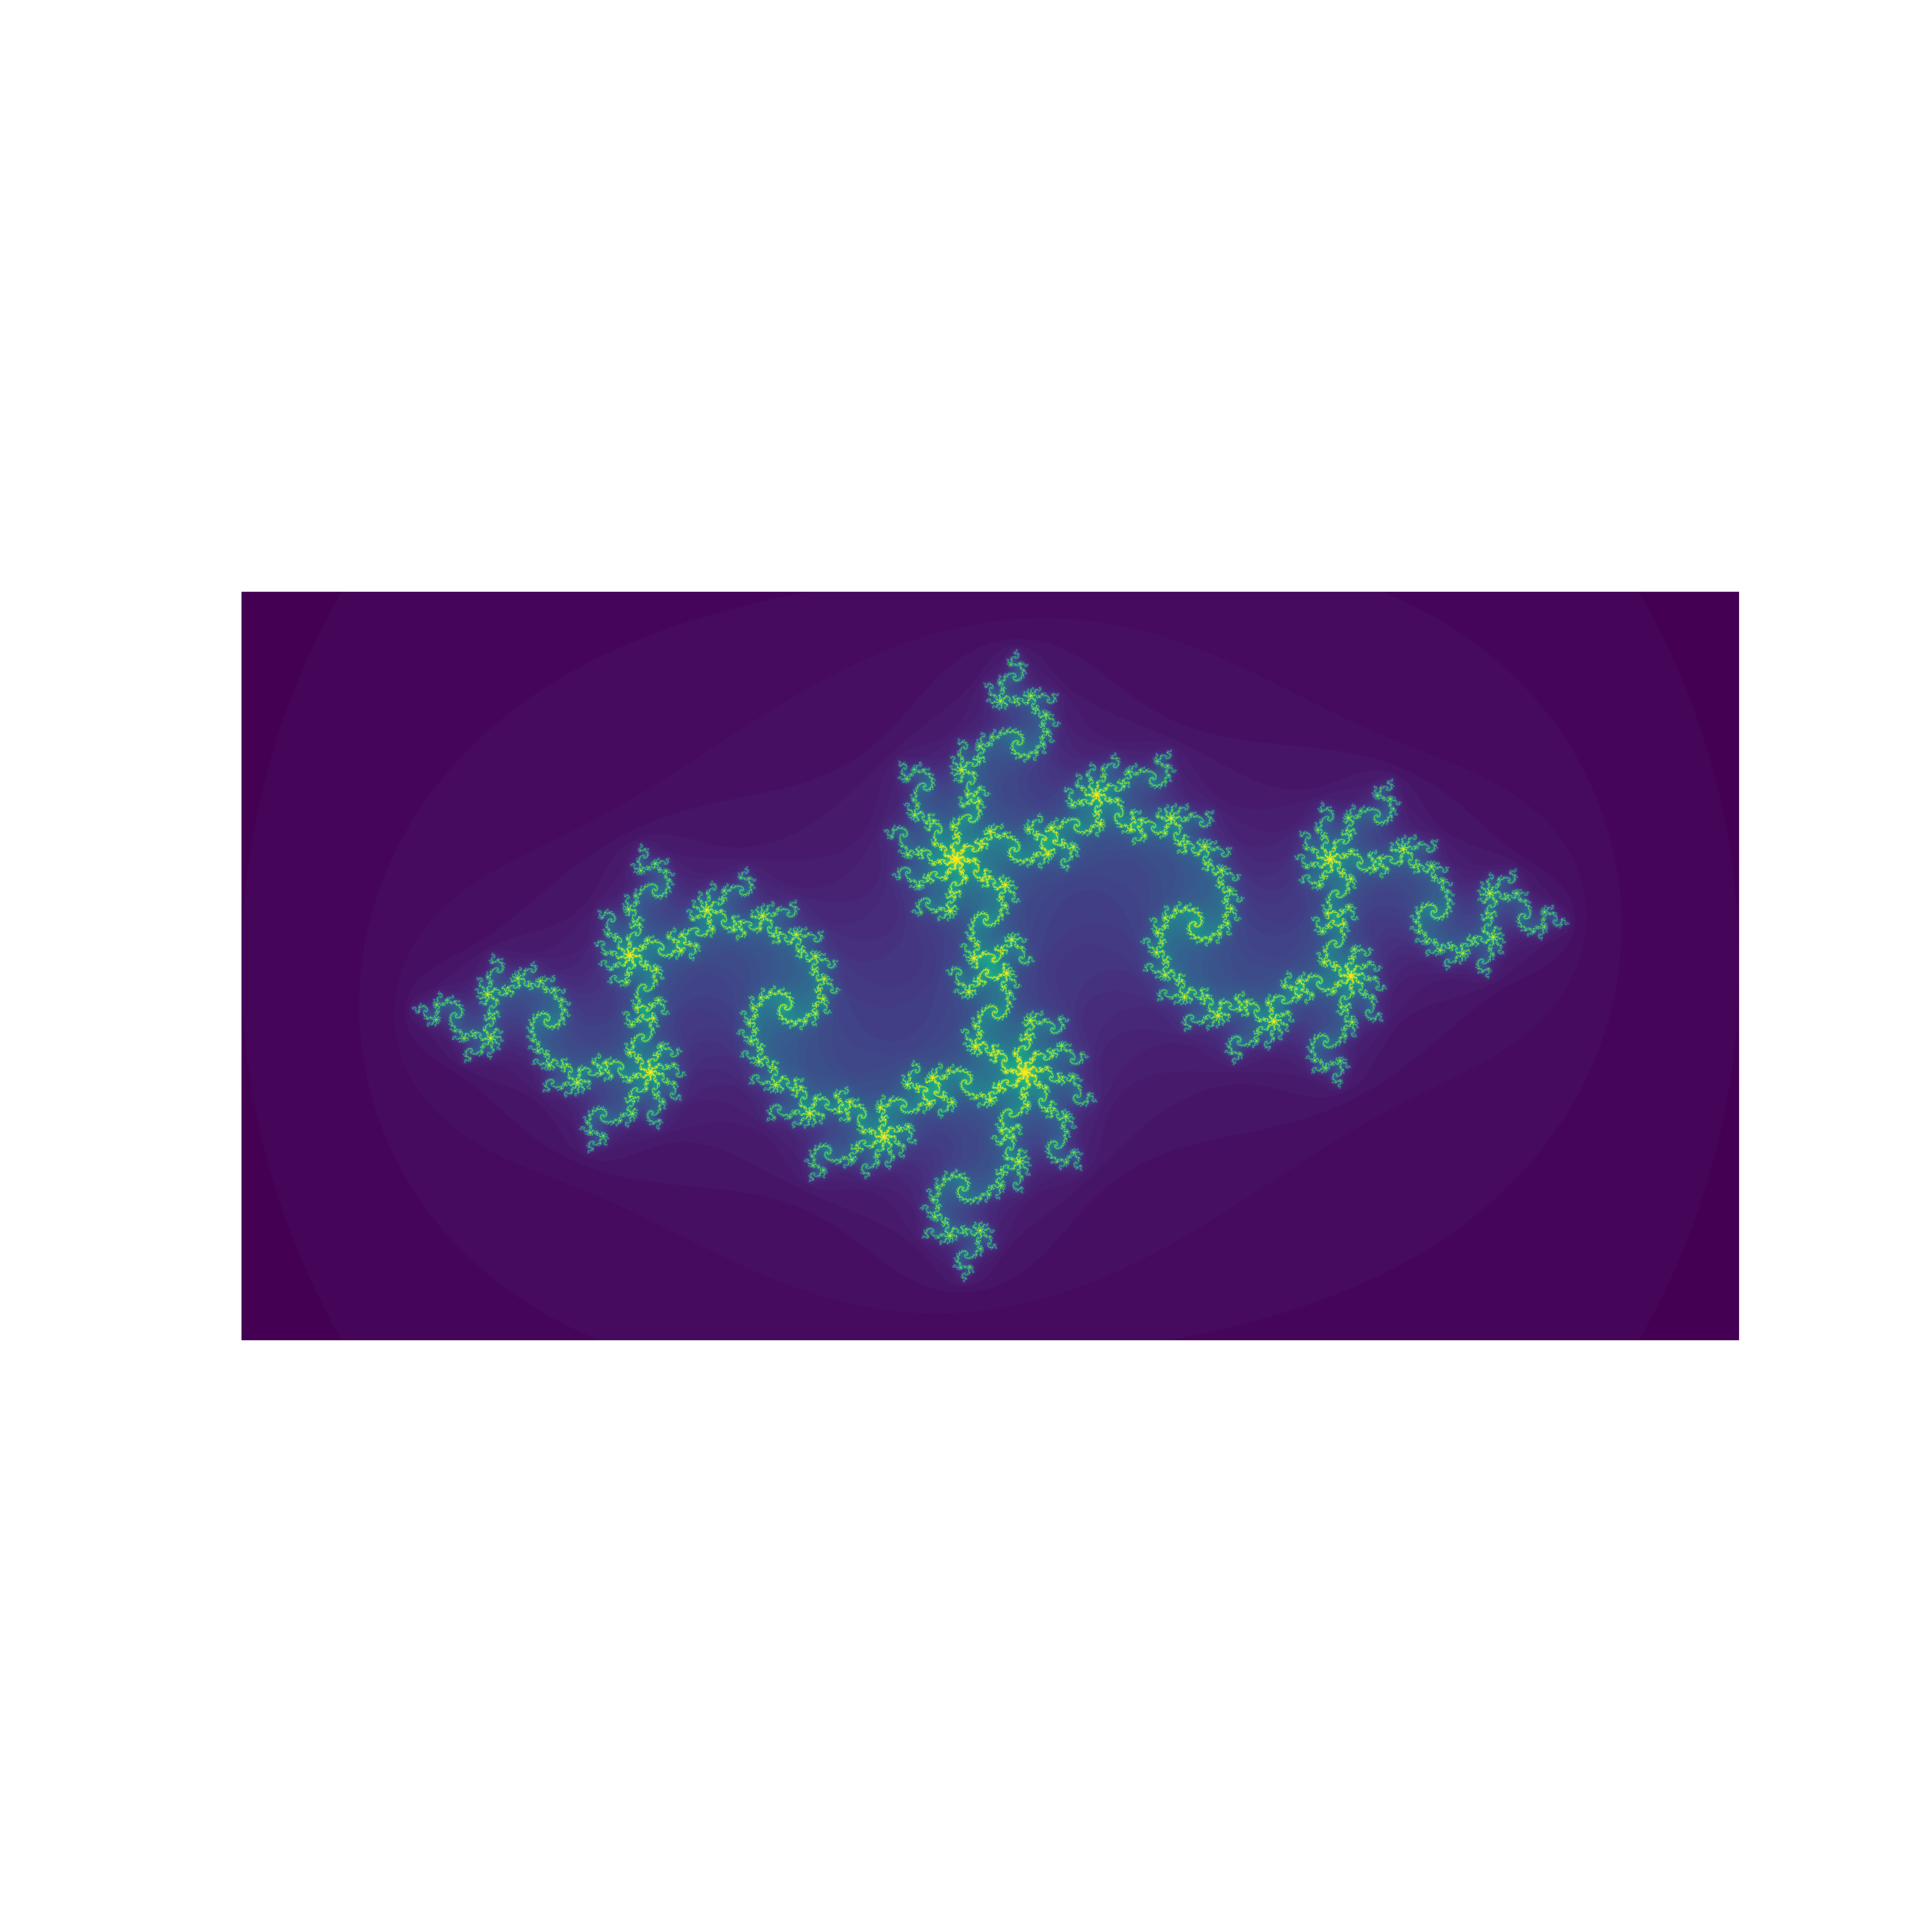
\includegraphics[width=\linewidth]{julia.png}
    \caption{Julia}
\end{figure}

\section{B}
\lipsum[2]


%\backmatter
%%%%% Bibliography %%%%%
\clearpage
\singlespacing
\nocite{*}
\printbibliography[heading=bibintoc]
%%%%%%%%%%%%%%%%%%%%%%%%

%%%%% Appendix %%%%% 
\clearpage
\appendix
%\addchap{}
\addcontentsline{toc}{chapter}{Appendix}
\centerline{\bf{Appendix}}
%\chapter{Appendix}
\singlespacing
%\refstepcounter{chapter}

\input{appendix/appendix.tex}

\end{document}
